\documentclass[xcolor=dvipsnames,hyperref={pdfpagelabels=false}]{beamer}

\usetheme{Boadilla}

\newcommand{\bi}{\begin{itemize}}
\newcommand{\ei}{\end{itemize}}
\newcommand{\be}{\begin{enumerate}}
\newcommand{\ee}{\end{enumerate}}
\newcommand{\bc}{\begin{center}}
\newcommand{\ec}{\end{center}}
\newcommand{\bd}{\begin{description}}
\newcommand{\ed}{\end{description}}
\newcommand{\I}{\item}
\newcommand{\f}{\frame}
\newcommand{\ft}{\frametitle}

\title{Offline Software Overview}
\subtitle{GlueX Collaboration Meeting}
\author[Mark Ito]{Mark M.\ Ito}
\date{May 13, 2014}
\institute[JLab]{Jefferson Lab}

\begin{document}

\f{\titlepage}

\f{\ft{Outline}
\bi
\I Data Challenge
  \bi
  \I goals
  \I conditions
  \I sites
  \I organization
  \I issues
  \I results
  \I outcomes
  \I next
  \ei
\I Other Topics
\I To Do
\ei
}

\f{\ft{Goals}
\bi
\I nominal goal 10 billion events.
\I Pythia/BGGEN events from 7.0GeV to the endpoint.
\I Target distribution to be nominal LH2 as handled by HDGEANT.
\I 1350 A current for magnetic field
\I updated REST format, matching info saved
\I use the CCDB
\I not crash so much
\ei
}
  
\f{\ft{Conditions}
\bi
\I software versions specified
\I background settings \\
\begin{tabular}{|c|c|c|}
\hline
Run & $\gamma$ Rate & fraction \\
\hline
9001 & $1\times 10^7$ & 80\% \\
9002 & $5\times 10^7$ & 5\% \\
9003 & 0 & 15\% \\
\hline
\end{tabular}
\I file number assignments for each site
\I configuration files specified
\I command-lines specified
\ei
}

\f{\ft{Conditions Webpage}
$$
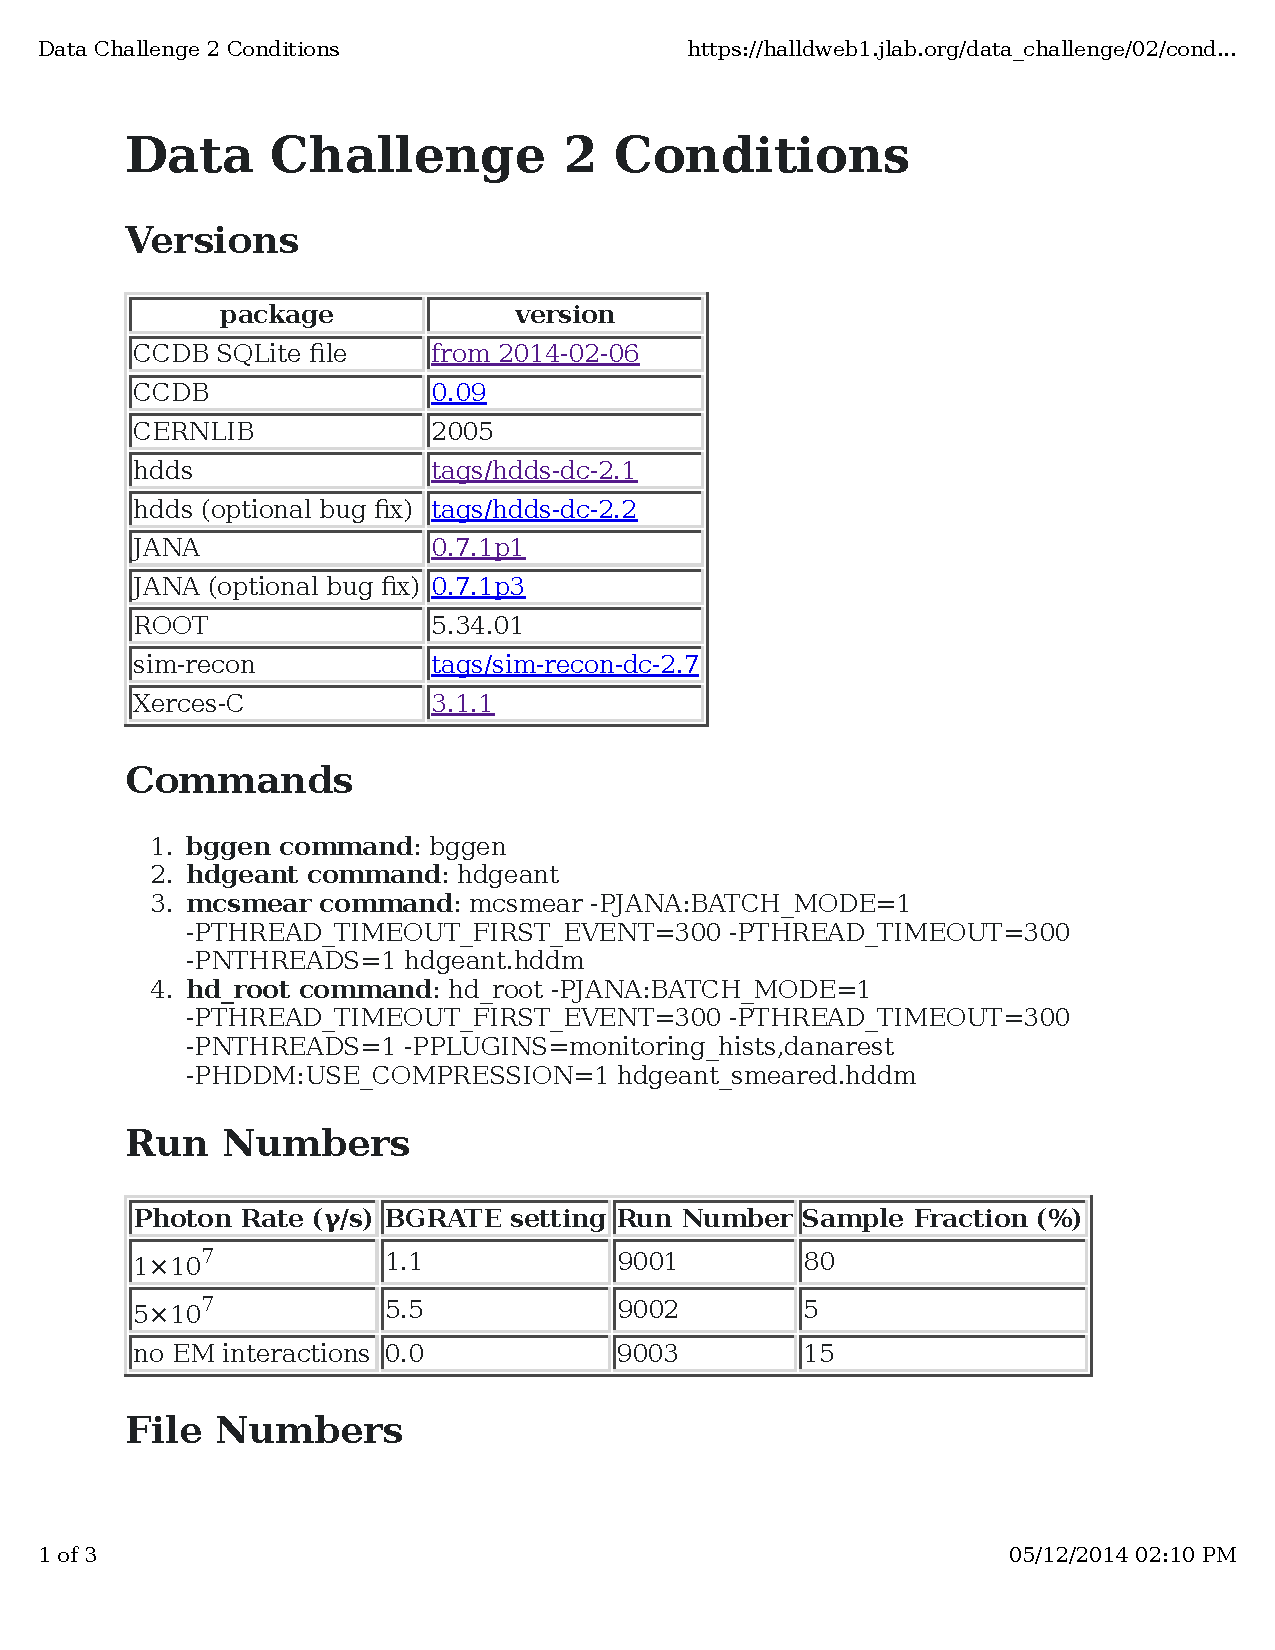
\includegraphics[height=0.9\textheight]{conditions.pdf}
$$
}

\f{\ft{Sites}
\bi
\I Carnegie Mellon
  \bi
  \I 384 cores
  \ei
\I Florida State
  \bi
  \I 144 cores
  \ei
\I JLab
  \bi
  \I 400 to 2400 cores
  \I workflow tools at JLab not ready
  \ei
\I MIT
  \bi
  \I 300+ cores
  \I OpenStack at MIT
    \bi
    \I Virtual Machines instances
    \I MIT Re-Use Cluster
    \I FutureGrid
    \ei
  \ei
\I Open Science Grid (OSG)
  \bi
  \I up to 10,000 cores
  \I nodes contributed from UConn and Northwestern
  \ei
\ei
}

\f{\ft{Organization}
\bi
\I Curtis initiated series of weekly meetings
  \bi
  \I 10 held: January 31 through April 11
  \I in addition to Offline meetings
  \ei
\I conditions webpage
  \bi
  \I Subversion controlled
  \ei
\I Event Tally Board
  \bi
  \I Google Drive spreadsheet
  \ei
\ei
}

\f{\ft{Issues}
\bi
\I reversed magnetic field fixes from Simon
\I Kei studied effect of EM background on file size, and execution time, varying beam rate and gate length
\I phi = 0 problem in CDC solved, Richard, Simon
\I event geneology checked by Kei
\I fix from Simon for single-ended TOF counters
\I improvements from Paul for cutting off processing for multi-lap curling tracks, big memory footprint effect
\I ZFATAL fix from richard, showers from EM background, squelched
\I short REST file fix from richard: bug in xstream library with compression enabled
\I non-reproducibility fixed: sort needed on associated objects in STL map
\ei
}

\f{\ft{Issues (continued)}
\bi
\I random number seeds
  \bi
  \I looked at scheme where every event stores its seed at each stage
  \I settled on bggen seed; concession to GEANT random number generator
  \ei
\I Kei studied EM background effect for $p\pi^+\pi^-$, $p\pi^+\pi^-\pi^0$
\I enhanced job tracking info at JLab added, MMI
\I Python script to scan monitoring histograms from Sean
\ei
}

\f{\ft{Results}
\bi
\I code frozen on March 20
\I events produced: more than 8 billion
\I execution time \\
\begin{tabular}{|c|c|c|}
\hline
Run & $\gamma$ Rate & sec/event \\
\hline
9001 & $1\times 10^7$ & 2.4 \\
9002 & $5\times 10^7$ & 9.0 \\
9003 & 0 & 0.75 \\
\hline
\end{tabular}
\I memory usage: about 1 GB peak virtual memory
\I reliability:
  \bi
  \I CMU: 7000 jobs, 3 failures
  \I JLab: 69,000 jobs, about 50 failures
  \ei
\I JLab node history:
  \bi
  \I Hall D share from 360 to 440 to 1440 to 2440
  \I Million core hours owed to us, cores lent to lattice QCD cluster
  \ei
\I non-OSG sites ramped down April 11 plus or minus a few days (last data challenge meeting)
\ei
}

\f{\ft{JLab Farm Usage}
$$
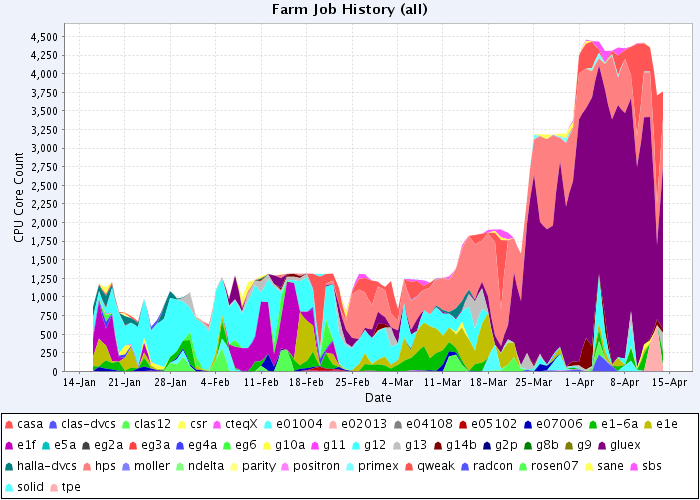
\includegraphics[width=0.9\textwidth]{Farm_2014.png}
$$
}

\f{\ft{MIT OpenStack Jobs}
$$
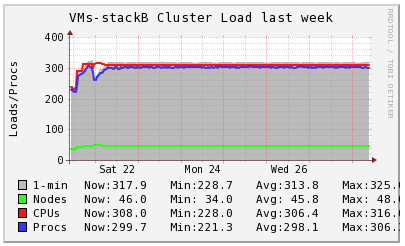
\includegraphics[width=0.9\textwidth]{MIT_DC2_3-28-14.png}
$$
}

\f{\ft{CPU Time Usage (Jlab)}
$$
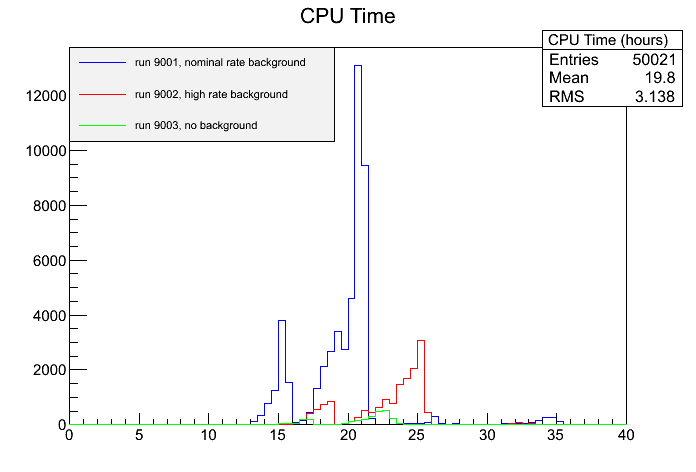
\includegraphics[width=0.9\textwidth]{cput.png}
$$
}

\f{\ft{Virtual Memory Peak (JLab)}
$$
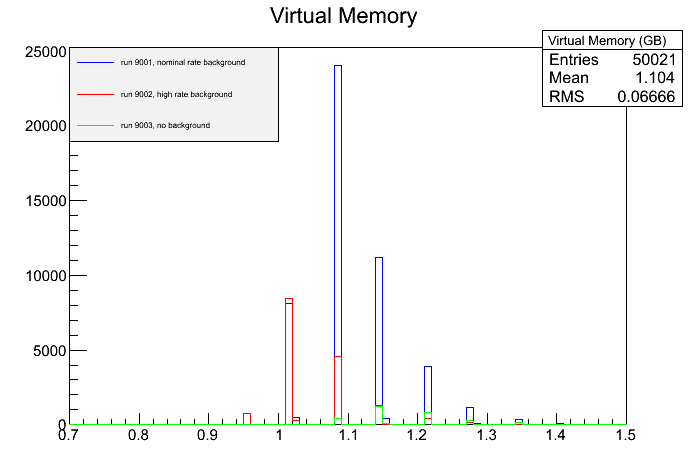
\includegraphics[width=0.9\textwidth]{vmem.png}
$$
}

\f{\ft{Data Distribution}
\bi
\I Storage Resource Manager (SRM)
  \bi
  \I go-to method for shipping data between sites
  \I archiving all data to tape library at JLab now
  \ei
\I EventStore
  \bi
  \I Sean developing this
  \I Multiple skim available from single data file (REST)
  \I Managing event lists
  \ei
\I Paul developed menu of skims we might do
\ei
}

\f{\ft{What Came Out}
\bi
\I need more efficient EM background generation scheme
\I large usable data set (hopefully)
\I improvements of techniques at various sites
\I need a monitoring system for production (ROOTSpy?)
\I need for Geant4
\ei
}

\f{\ft{Next Data Challenge}
\bi
\I stage ``raw data'' on tape library
\I ``production''
\I tape overhead
\I test multi-threading
\I needed: raw data, ability to analyze it
\I summer?
\ei
}

\f{\ft{Other Topics}
\bi
\I CCDB 1.00 released
\I kinematic fitter update
\I nightly build using scons
\I BlueJeans deployed
\I splitting up offline packages
\I re-org of offline wiki pages
\ei
}

\f{\ft{Conclusions}
\bi
\I much more robust software suite coming out of data challenge
\I high level of cooperation and coordination demonstrated
\I lots to do
\I next frontier: reconstruction quality
\ei
}

\end{document}
